\section*{Introduction} % Pas de numérotation
\addcontentsline{toc}{section}{Introduction} % Ajout dans la table des matières
	En lisant le titre de ce rapport, vous avez pu vous demander : "Mais qu'est-ce que Ace Attorney ?" .\newline
	Ace Attorney est une série de jeux vidéos développés par Capcom et édités par Nintendo depuis 2001 sur GameBoy Advance puis portée sur DS et 3DS.\newline
	Ce type de jeu est le visual novel, c'est-à-dire que l'aventure du jeu se défile sous nos yeux, en superposant du texte, qui sera alors le script du jeu, sur une image de fond. Le joueur doit, à certains moments, agir afin de faire avancer l'action du jeu.\newline
	Dans ces jeux, nous incarnons un avocat à la défense, qui doit prouver l'innocence de ses clients en découvrant la vérité sur l'affaire en cours (généralement un meurtre).\newline
	Ces jeux se déroulent en deux phases: une d'enquête, où l'on cherche des preuves afin de disculper notre client, et une phase de procès où nous confrontons les preuves accumulées aux différents témoignages pour déméler le vrai du faux et ainsi résoudre l'affaire.\newline
	
	Dans ce projet, nous n'avons implémenté que la première affaire du premier jeu (The First Turnabout) qui ne contient qu'une phase de procès.\newline
	
	Nous décrirons dans un premier temps les raisons qui nous ont poussées à faire ce projet, puis nous détaillerons les structures et algorithmes utilisés pour la partie graphique (OpenGL), ensuite nous expliciterons les structures et algorithmes de la partie script. Nous finirons par exprimer les différents problèmes rencontrés, les idées d'améliorations et nous conclurons.
	
\begin{figure}[!ht]
	\centering
	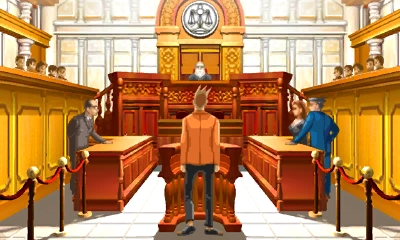
\includegraphics [width=10cm]{images/aa_screen_original.jpg}
	\caption{Un aperçu du jeu original}
	\label {screen_game}
\end{figure}